\documentclass{article}
\usepackage{ctex}
\usepackage{graphicx}
\usepackage{amsmath}
\usepackage{geometry}
\usepackage{float}
\geometry{a4paper, margin=1in}

\title{\textbf{系统开发工具基础\_实验报告（第3周）}}
\author{李雨潼 \\ 25020007069}
\date{}

\begin{document}

\maketitle

\section*{一、课上实验题}

\subsection*{第9题：从源码构建并在干净环境安装Wheel}
\textbf{题目要求：} 在 q09 中按给定内容创建 Python 命令行包，运行 python -m build 生成 wheel，在干净虚拟环境中安装，运行 sdt-greet --name <学号> 确认输出正确。

\textbf{执行结果：}
\begin{figure}[H]
    \centering
    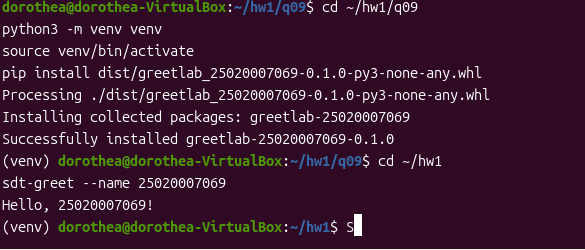
\includegraphics[width=0.9\textwidth]{q9.png}
    \caption{第9题执行结果（sdt-greet 运行输出）}
    \label{fig:q9}
\end{figure}

\newpage

\subsection*{第10题：让编程智能体进入可验证的修复循环}
\textbf{题目要求：} 复制 q09 为 q10，添加一个失败测试：当 name 只含空白字符时，main 应以 SystemExit(2) 结束。先运行测试确认失败，向编程智能体说明目标并修改实现，人工检查 diff 后再次运行测试。

\textbf{执行结果：}

测试失败（修改前）：
\begin{figure}[H]
    \centering
    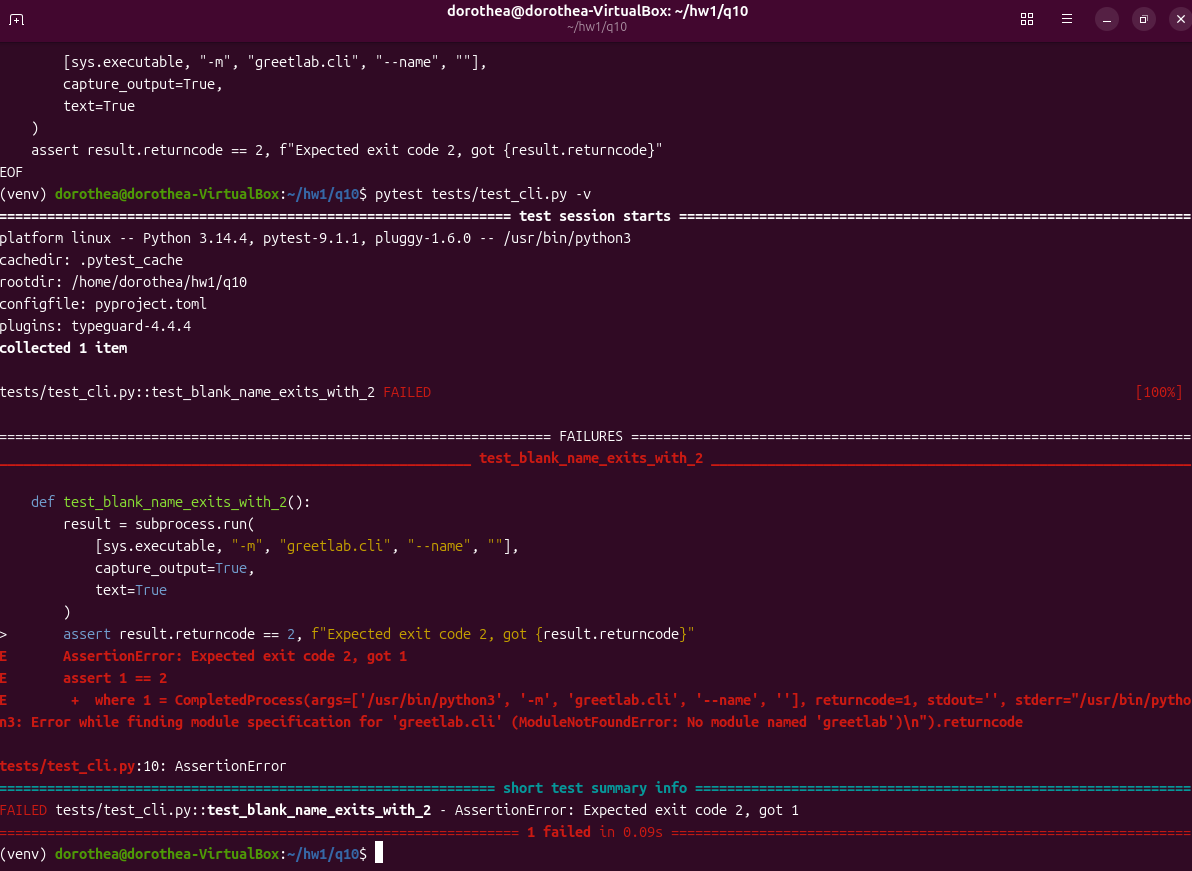
\includegraphics[width=0.9\textwidth]{q10_1.png}
    \caption{测试失败：空 --name 返回码为 0，不符合预期}
    \label{fig:q10_1}
\end{figure}

测试通过（修改后）：
\begin{figure}[H]
    \centering
    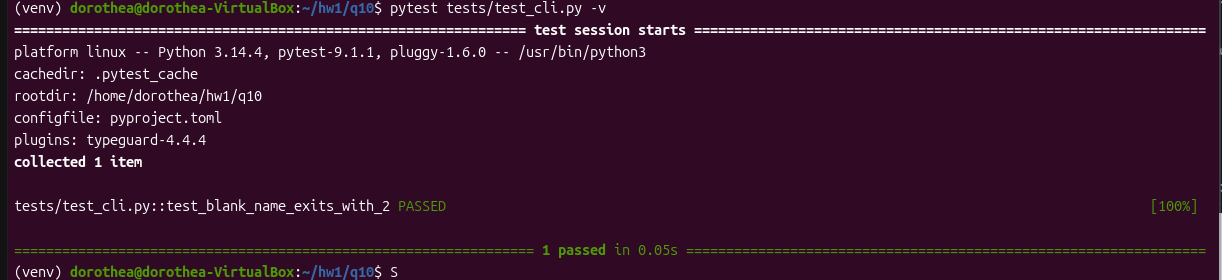
\includegraphics[width=0.9\textwidth]{q10_2.png}
    \caption{测试通过：空 --name 返回码为 2，符合预期}
    \label{fig:q10_2}
\end{figure}

ai\_log.md 记录：
\begin{figure}[H]
    \centering
    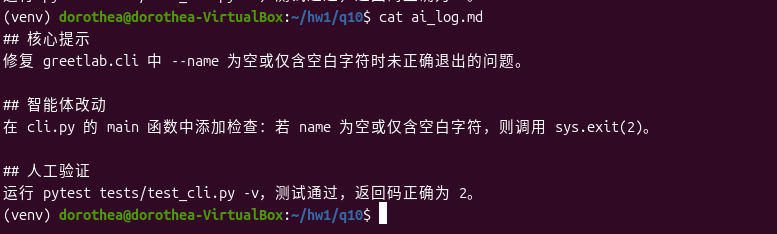
\includegraphics[width=0.9\textwidth]{q10_3.png}
    \caption{ai\_log.md 内容（核心提示、智能体改动、人工验证）}
    \label{fig:q10_3}
\end{figure}

\newpage

\subsection*{第11题：把“无法处理”的协作材料改成可执行信息}
\textbf{题目要求：} 在 communication.md 中重写 Issue、提交信息和评审意见，包含环境、复现命令、期望结果和实际结果，全文 400 字以内。

\textbf{执行结果：}
\begin{figure}[H]
    \centering
    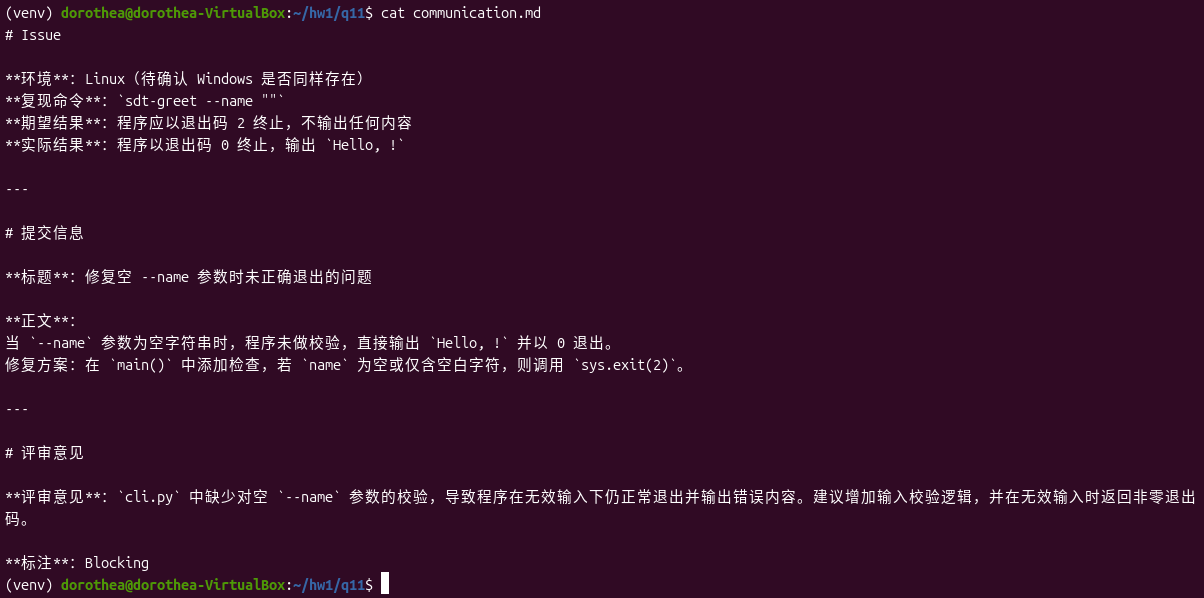
\includegraphics[width=0.9\textwidth]{q11.png}
    \caption{communication.md 内容}
    \label{fig:q11}
\end{figure}

\newpage

\subsection*{第12题：修复一个可复现的线性回归训练循环}
\textbf{题目要求：} 补全训练循环（zero\_grad、backward、step），调用 model.eval()，在 torch.no\_grad() 中打印最终损失、weight 和 bias，损失应小于 0.001。

\textbf{执行结果：}
\begin{figure}[H]
    \centering
    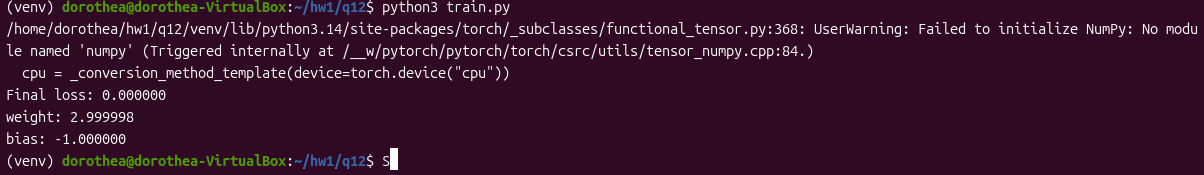
\includegraphics[width=0.9\textwidth]{q12.png}
    \caption{训练结果：最终损失 0.000000，weight 2.999998，bias -1.000000}
    \label{fig:q12}
\end{figure}

\newpage

\section*{二、课后练习（10个实例）}

\subsection*{实例1：虚拟环境环境变量变化}
创建并激活 venv，对比环境变量变化。
\begin{figure}[H]
    \centering
    
\includegraphics[width=0.9\textwidth]{ex1.png}
    \caption{实例1执行结果}
    \label{fig:ex1}
\end{figure}

\subsection*{实例2：创建Python包并在venv中安装}
编写 pyproject.toml，使用 pip install -e . 安装包。
\begin{figure}[H]
    \centering
    
\includegraphics[width=0.9\textwidth]{ex2.png}
    \caption{实例2执行结果}
    \label{fig:ex2}
\end{figure}

\subsection*{实例3：生成锁文件（lock file）}
使用 pip freeze 生成 requirements.txt 锁文件。
\begin{figure}[H]
    \centering
    
\includegraphics[width=0.9\textwidth]{ex3.png}
    \caption{实例3执行结果}
    \label{fig:ex3}
\end{figure}

\subsection*{实例4：斐波那契数列}
用递归实现斐波那契数列并运行。
\begin{figure}[H]
    \centering
    
\includegraphics[width=0.9\textwidth]{ex4.png}
    \caption{实例4执行结果}
    \label{fig:ex4}
\end{figure}

\subsection*{实例5：查看项目结构}
使用 ls -la 查看当前目录下项目结构。
\begin{figure}[H]
    \centering
    
\includegraphics[width=0.9\textwidth]{ex5.png}
    \caption{实例5执行结果}
    \label{fig:ex5}
\end{figure}

\subsection*{实例6：命令行计算器}
用 AI 编写简单的命令行计算器，支持加减乘除。
\begin{figure}[H]
    \centering
    
\includegraphics[width=0.9\textwidth]{ex6.png}
    \caption{实例6执行结果}
    \label{fig:ex6}
\end{figure}

\subsection*{实例7：查看本地 Git 提交历史}
使用 git log --oneline --graph 查看提交历史。
\begin{figure}[H]
    \centering
    
\includegraphics[width=0.9\textwidth]{ex7.png}
    \caption{实例7执行结果}
    \label{fig:ex7}
\end{figure}

\subsection*{实例8：查找 good first issue}
在 GitHub 上查找带 good first issue 标签的 Issue，截图搜索结果。
\begin{figure}[H]
    \centering
    
\includegraphics[width=0.9\textwidth]{ex8.png}
    \caption{实例8执行结果}
    \label{fig:ex8}
\end{figure}

\subsection*{实例9：最小可复现示例}
编写一个会触发 ZeroDivisionError 的最小程序。
\begin{figure}[H]
    \centering
    
\includegraphics[width=0.9\textwidth]{ex9.png}
    \caption{实例9执行结果}
    \label{fig:ex9}
\end{figure}

\subsection*{实例10：解释陌生代码库}
查看 mypackage 包结构，解释 \_\_init\_\_.py 中的 hello 函数。
\begin{figure}[H]
    \centering
    
\includegraphics[width=0.9\textwidth]{ex10.png}
    \caption{实例10执行结果}
    \label{fig:ex10}
\end{figure}

\section*{三、解题感悟}

本次实验涵盖了打包工具、智能体编程、协作规范和 PyTorch 训练四个主题。

第9题让我完整走了一遍从编写 Python 包到构建 wheel 再到虚拟环境安装的流程，对 setuptools 和 pyproject.toml 的用法有了更具体的认识。第10题在第9题的基础上添加了测试，用 AI 智能体辅助修复了输入校验问题，体验了测试驱动的修改方式。第11题是协作材料改写，把不规范的 Issue 和提交信息改成更专业的表达，这种能力在实际工作中比较实用。第12题补全了 PyTorch 的训练循环，通过 zero_grad、backward 和 step 完成了线性回归训练。

课后10个实例练习了虚拟环境、包管理、Git 历史查看、最小可复现示例等，这些工具在日常开发中经常用到。整体来说，这一周的内容更偏向实际工程开发，让我对打包和协作流程有了更具体的印象。

\end{document}